%describe the background necessary to understand the lab's content, with some reservation (i.e., not too much detail)
%possibly provide walkthrough for simple problem
\section{Introduction}

The purpose of this lab is to introduce and learn the concept of object interaction. An object consists of data and methods grouped together to form an entity. It also has a sort of "object interface" which consists of methods that define how the object will interact with other objects.

\noindent
For this lab, you will be developing two classes: a CameraActivity and an EditActivity class. The camera capabilities on the Android phone will be utilized. You will be required to code each of these objects in a way that they can interact with each other to accomplish the task of capturing a picture and editing that picture.

\noindent
The CameraActivity class should be able to take a picture with the camera, and then send it to the EditActivity class to be maniplulated by the user.

\noindent
In this lab, you will be required to use certain classes from the Android SDK API. Here is a list of things you will need to research before beginning:

\begin{itemize}
	\item android.content.Intent
	\item android.graphics.Bitmap
	\item android.net.Uri
	\item android.provider.MediaStore
	\item android.widget.ImageView
\end{itemize}

\begin{center}
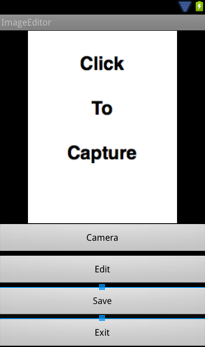
\includegraphics[scale=0.4]{screenshot.png} 
\end{center}
